\documentclass{standalone}

\begin{document}

\chapter*{Appendix D - Multi-Class Performances}\addcontentsline{toc}{chapter}{Appendix C - Multi-Class Performances}
\markboth{Appendix D}{Scorer}

\begin{center}
\begin{figure}[htbp]
\centering
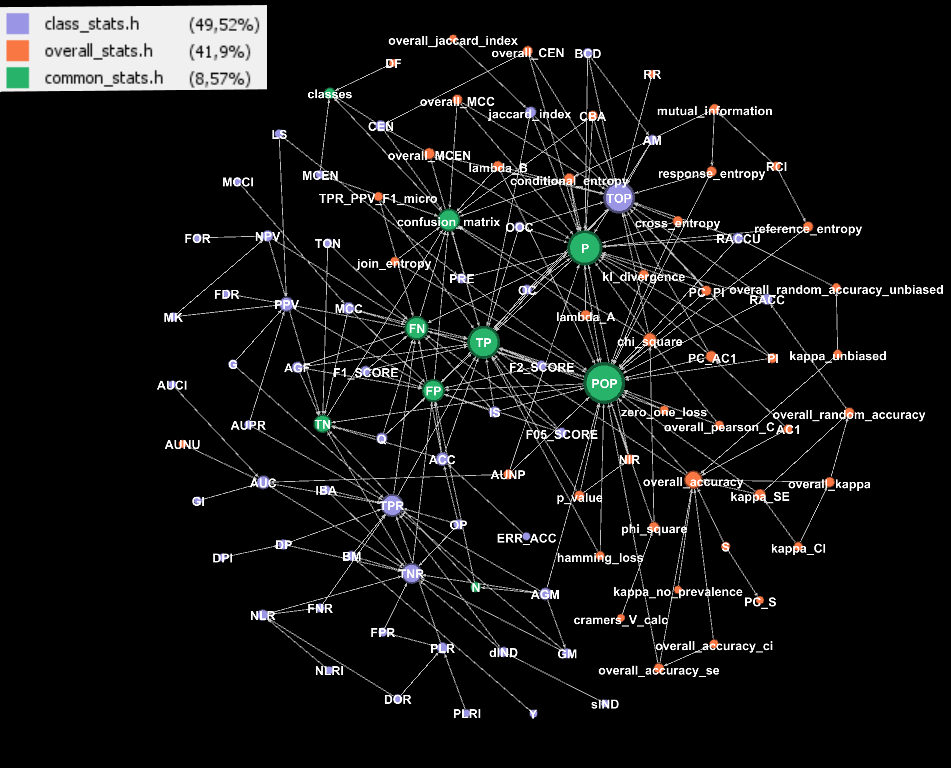
\includegraphics[width=0.6\textwidth]{scorer_net.png}
\caption{Multi class score interaction graph.
Each node identifies a different performance evaluator and links are given by the interactions between mathematical formulations of each quantity.
The graph has more than 100 nodes and more than 200 links.
The node colors are given by the classes identified in the work of Sepand et al.~\cite{PyCM}.
}
\label{fig:scorer_net}
\end{figure}
\end{center}

The performances evaluation is a crucial task in any Machine Learning application.
Given a set of patterns and its corresponding (true) labels we can evaluate the efficiency of a given model with a comparison between labels and model outputs, i.e the predicted labels.
There are a lot of different score functions that can be computed and any of them evaluates some aspects of the model efficiency.
Any paper author choses the score that better highlights the advantages of its model and it is difficult to move around this large zoo of indicators.
Moreover, (it is quite a constant in scientific research) when a paper is send to a peer-review, in many cases the reviewers suggest to check if other performance indicators are good enough for the showed results.
This means that a lot of large simulations should be performed again and the appropriated variables recomputed to obtain the requested scores.

At this point the main question is: are these scores totally independent one from each other?
The brief answer is simply no.
In a very interesting work of Sepand et al.~\cite{PyCM} the authors show how we can compute a wide range of these scores starting from the evaluation of the simple confusion matrix\footnote{
  The confusion matrix is a square matrix of shapes $(N, N)$, with $N$ the total number of classes in the current problem, whose entries are the number of right and false classifications.
  In particular, each entry of the matrix represents the predicted instances in a given class.
  If the class is the right one we call it as true positive item.
  As counterpart we have a false positive item.
}, providing a full mathematical documentation and references about their numerical evaluation.

Despite the \textsf{Python} code provided by Sepand et al. explains these links between the mathematical quantities they stop their analyses on the score evaluations without any interest on the optimization of these computations.
Starting from their work we analyzed the inter-connections between these mathematical formulas and we extracted the dependencies between the involved variables.
In particular, a score function can be interpreted as a node and its connections could be given by the variables needed to evaluate it.
This type of graphs are commonly called \href{https://en.wikipedia.org/wiki/Factor_graph}{\emph{factor graphs}}.
In a mathematical formulation of \emph{factor graphs} there are different kinds of nodes (variables and factors, or equations).
The focus of our analysis was not on mathematical formalism of these kind of graphs but we aimed to a visualization of function interactions and an analysis of the numerical improvements derived from it.

In the work of Sepand et al. the authors identify three function classes: common statistics, class statistics and overall stats.
In Fig.~\ref{fig:scorer_net} the interaction graph of these three classes is shown.
The figure shows deep interactions between the three function classes and it highlights the dependencies of the different quantities involved.
We can also use this kind of visualization to formulate computational considerations about the order in which these quantities could be evaluated.
Since the graph is a direct graph by definition, we can start from the root node (the node without links which bring to it) and cross the network until the leaf nodes (nodes without link which go out from them) like in a tree-graph.
At each step of the percolation, the incoming nodes identify totally independent quantities.
This independence means that the nodes-quantities can be potentially computed in parallel.
To clarify this consideration we can reorganize the graph visualization minimizing the link lengths and obtaining a stratified graph in which each level identifies a potential parallel section.
A graph with these properties was obtained using the \textsf{dot} visualization and it is shown in Fig.~\ref{fig:scorer_parallel}.
As can be seen in figure we can identify 7 levels in the graph and thus 7 potential parallel regions for the computation of the full set of functions.

\begin{center}
\begin{figure}[htbp]
\hspace{-2cm}

\includegraphics[width=1.3\textwidth]{scorer_parallel.pdf}
\caption{Re-organization of the graph in Fig.~\ref{fig:scorer_net}.
The rendering was obtained using the \textsf{dot} visualization, i.e the minimization of the link lengths.
The direct graph identifies the tree of dependencies and each level of the tree represents a set of independent functions that can be potentially computed in parallel.
This graph is used as parallel scheme for the \textsf{Scorer} library.
}
\label{fig:scorer_parallel}
\end{figure}
\end{center}

These considerations allow us to create an optimized version of the code of Sepand et al., the \textsf{Scorer} library~\cite{Scorer}.
The \textsf{Scorer} library is the \textsf{C++} porting of the \textsf{PyCM} library of Sepand et al. with a \textsf{Cython} wrap for the \textsf{Python} compatibility.
Following the above told graph the computation of score quantities are performed in parallel according to the 7 levels found.
The parallelization strategy chosen uses the \textsf{section} keywords of OpenMP library to perform no-wait tasks that are computed by each thread of the parallel region.

The extracted graph includes more than 100 different quantities so writing the full set of parallel sections becomes an hard (boring) work in \textsf{C++}.
Moreover, update the graph with new quantities brings to a consequential update of the full code and also of the parallelization strategy.
Each function was written as an anonymous-struct, i.e a functor, with an appropriate operator overloading.
Each functor has a name given by a pre-determined regex (\textsf{get\_\{function\}}) and the list of arguments follows the same nomenclature\footnote{
  If the functor receives in input the variable $A$ and $B$ we have to ensures that two functors named $get\_A$ and $get\_B$ will be provided.
  The only exception is given by the root functor.
}.
With these expedients we created a fully automated \textsf{C++} script which parses the list of functors, it computes the dependency graph and the parallelization levels and it gives back a compilable \textsf{C++} script with the desired characteristics.
In this way we can guarantee an easy way to update the library and moreover we overcome the boring writing of a long code.
The automatic creation script is provided in the \textsf{Scorer} library and it should be used at each pull request or version update.

For a pretty/useful visualization of the computed quantities we rendered the interaction graph in an HTML framework.
In this way we can insert with a CSS table the computed values in each node that can be discovered passing the mouse over the figure.
An example of this rendering is given in the on-line version of the library~\cite{Scorer}.

In conclusion the developed \textsf{Scorer} library is a very powerful tool for Machine Learning performances evaluation which can be used either in \textsf{C++} either in \textsf{Python} codes through the \textsf{Cython} wrap.
The code is automatically generated at each update and automatically tested using continuous integration for any platform using \href{https://github.com/Nico-Curti/scorer/blob/master/.travis.yml}{Travis CI} and \href{https://github.com/Nico-Curti/scorer/blob/master/appveyor.yml}{Appveyor CI}\footnote{
  We perform tests for Unix and Windows environments.
  We check more than 15 combinations of environments and compilers.
}.
The code can be compiled using \href{https://github.com/Nico-Curti/scorer/blob/master/CMakeLists.txt}{\textsf{CMakefile}} or \href{https://github.com/Nico-Curti/scorer/blob/master/Makefile}{\textsf{Makefile}} and a \href{https://github.com/Nico-Curti/scorer/blob/master/setup.py}{\textsf{setup.py}} is provided for the \textsf{Python} version.
So when you write a new paper on Machine Learning and you do not know what could be the most appropriate indicator to show in your research or you are afraid that a referee could ask you to compute an other one there is only one solution: compute them all using \textsf{Scorer}.


\end{document}
